\section{Algoritmos de disparo del detector de superficie} \label{triggers_caracteristicas}

\subsection{Disparo Estándar}

El disparo ToT o \emph{Time over Threshold} está diseñado para adquirir datos de una duración relativamente larga, de esta manera se puede distinguir señales producidas por EASs por encima del ruido, ya que el último consiste en picos más cortos. Las señales producidas por un evento tienen un decaimiento exponencial con una constante de $70\,$ns, que es el tiempo de decaimiento de la luz dentro del tanque. Los PMTs registran señales en intervalos de $25\,$ns, por lo que una señal alta puede ser registrada durante varios periodos de adquisición de datos. Si por algún motivo, ya sea ruido u otro evento dentro de la ventana del disparo, se produce otro pico durante el decaimiento de la señal de evento puede cumplir la condición de disparo con una mayor señal que la que le corresponde. También existe el disparo \emph{Threshold} que no tiene la condición de las ventanas temporales del PMT sino que dispara cuando la señal pasa un umbral

{El eventos comúnmente presentados en los trabajos de la Colaboración Auger son registrados con un algoritmo de disparo ToT que se menciona como \emph{Disparo Estándar}.  Estos eventos son medidos utilizando un algoritmo cuya eficiencia varía con la energía del CR. Para el Disparo Estándar, los eventos con energía mayor a $3\,$EeV y ángulo cenital $\theta<60^o$ o  por encima de $4\,$EeV y $\theta<80^o$, son detectados con una eficiencia del 100\%. Por lo tanto, el análisis en el rango de energía entre $1\,$EeV - $2\,$EeV requiere factores relacionados con la eficiencia del disparo en función de la energía. Estos factores son obtenidos de manera fenomenológica \cite{taborda}.}


A medida que los tanques pasan más tiempo midiendo van perdiendo sensibilidad a los eventos de bajas energías. Esto es una desventaja del Disparo Estándar en los SDs en el rango $1\,$EeV - $2\,$EeV.  En la Fig.\ref{fig:futuro}, para los datos presentados en el ICRC 2019, se observa como la cantidad de eventos para energía menores a $3\,$EeV va disminuyendo, además la energía media de los eventos para distintos rangos de tiempo va aumentando.

 
\subsection{Todos los Disparos}

Para recuperar la sensibilidad para bajas energías, a partir del año 2013  se implementan otros algoritmos de disparo en los SDs, llamados ToTd y MoPS \cite{pierre2013plans}. Estos algoritmos de disparo se mencionan en este trabajo como \textit{Todos los Disparos}. A comparación del Disparo Estándar o ToT, el algoritmo ToTd hace una deconvolución del pico medido por el PMT. De esta forma se acelera la caída exponencial de la señal de un evento, y la reduce a uno o dos periodos de  $25\,$ns con una señal alta, seguida de varios picos con valores negativos \cite{ToTd}. En el caso de MoPS, el mismo cuenta la  cantidad de aumentos sucesivos en la señal detectada por el PMT en una ventana de tiempo dado. La condición de disparo se cumple si esta cantidad de aumentos sucesivos está por encima de cierto número \cite{MoPS}. El algoritmo MoPS es más sensible a las señales electromagnéticas, que son anchas en tiempo, en cambio el algoritmo ToTd es sensible a los picos de corta duración.  

% We first define apositive stepin a FADC trace as a cumulation of successive increases.  Thisis illustrated in Fig.1, where the positive steps are indicated by blue arrows.  Their valuesare  integer  by  definition.   The  MoPS  algorithm  consists  in  counting  how  many  positive steps exceed a certainthresholdThwithin a slidingwindowof a certain lengthW, and to require this number to be above a certainoccupancyvalueM.  So, the parameters definingthe trigger condition are similar to those defining the ToT trigger, except that hereThisdirectly defined in FADC units, not as a given fraction of a calibrated VEM value.
% suppresses the exponentialtail of an elementary signal and reduces it to one or two slots with high amplitude, followedby a tail of positive or negative values
% In case of the MoPS the trigger probability reaches a plateau of about 50\% asby design it is not sensitive to narrow peaks but to the spread electromagnetic signals

En la Fig.\ref{fig:TLD} se observa como la cantidad de eventos para energía menores a $3\,$EeV va disminuyendo como el caso del Disparo Estándar pero en una menor proporción con respecto a los eventos registrados con eficiencia completa. También se ve que en cada año activo de Todos los Disparos, hay un proporción más alta de eventos por encima de $3\,$EeV que con el Disparo Estándar.


\begin{figure}[H]
	\centering
	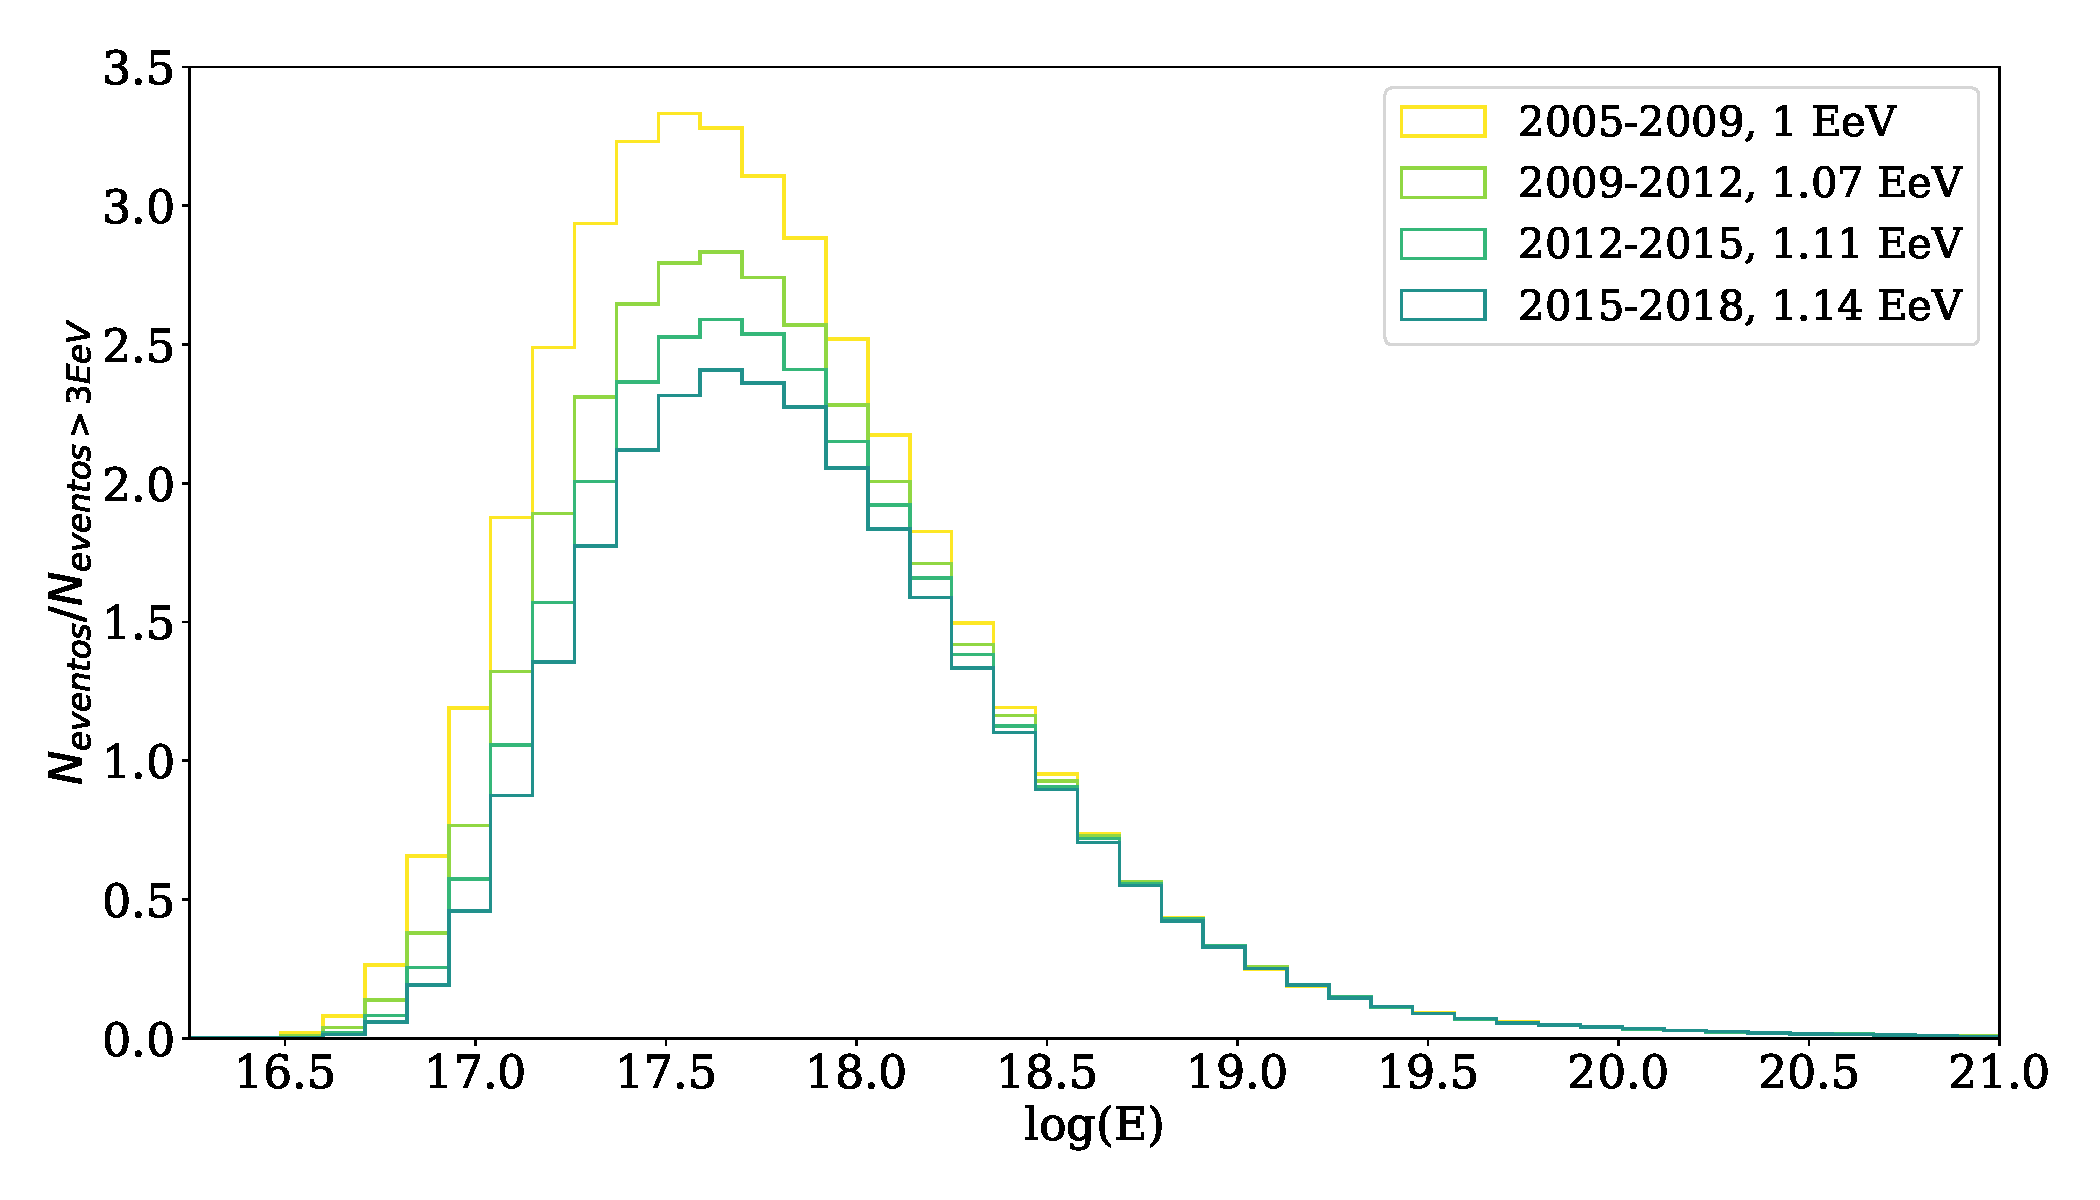
\includegraphics[width=0.8\textwidth]{histograma_Standard.pdf}
	\caption{Histograma de eventos  del Disparo Estándar por rango de tiempo medido por el Observatorio Pierre Auger. También se reporta la energía media el mismo rango de tiempo.}
	\label{fig:futuro}
\end{figure}


\begin{figure}[H]
	\centering
	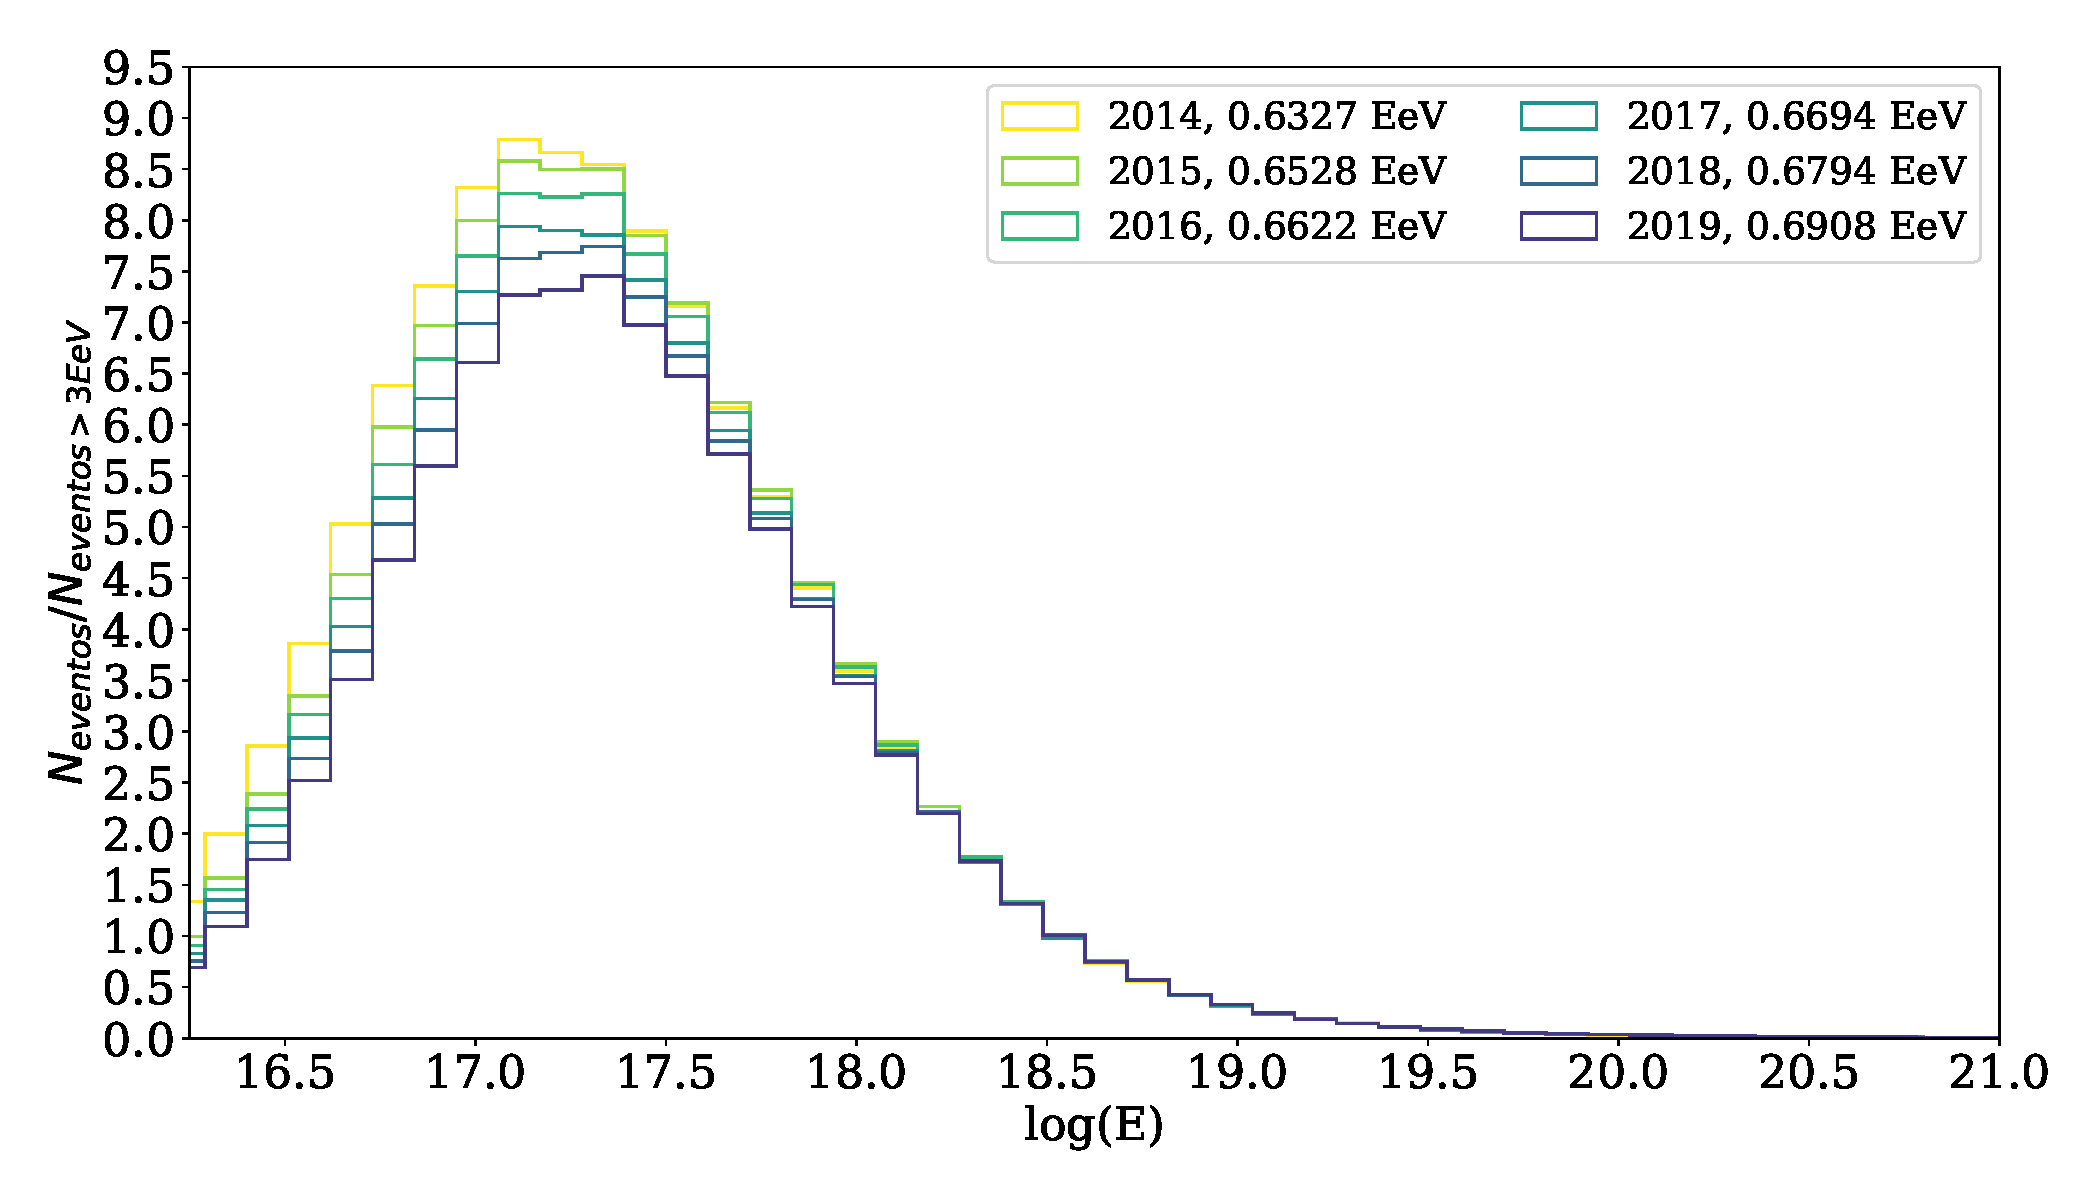
\includegraphics[width=0.8\textwidth]{histograma_AllTriggers_v2.pdf}
  \caption{Histograma de eventos de  Todos Los Disparos por cada año medido por el Observatorio Pierre Auger y sus respectiva energía media. }
	\label{fig:TLD}
\end{figure}

La implementación de los ToTd y MoPS fue llevada a cabo mediante una actualización de la electrónica de los SDs para bajar el umbral de disparo, en particular para las señales de la componente electromagnética de la EAS, mejorando así la reconstrucción de eventos mediante la separación fotón/hadrón para bajas energías  \cite{pierre2013plans}. Con esta mejora, el umbral de eficiencia completa para Todos los Disparos es menor que el Disparo Estándar, este umbral es de una energía de $1\,$EeV. En la Fig\,\ref{fig:triggers} se comparan las eficiencia del Disparo Estándar y Todos los Disparos en función de la energía del evento. De tal manera que, al estudiar los eventos en el rango $1\,$EeV - $2\,$EeV,  no son necesarios los factores de eficiencia y sólo pueden afectar los cambios de la exposición direccional del Observatorio.


\begin{figure}[H]
  \centering
  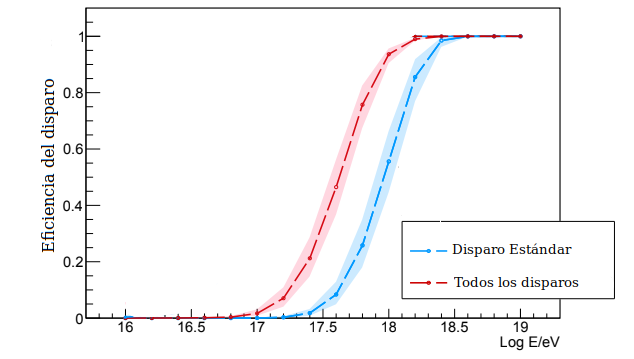
\includegraphics[width=0.75\textwidth]{comparacion_triggers.png}
  \caption{La eficiencia del disparo en función de la energía para eventos con ángulo cenital $\theta$ menor a $60^o$. Esta figura fue extraída de un trabajo interno de la Colaboración {\cite{triggers_ref}}.}
  \label{fig:triggers}
\end{figure}


Una desventaja de Todos los Disparos sobre el Disparo Estándar, es que el último tiene una mayor cantidad de años medidos, ya que se adquieren datos  desde el año 2004 con este algoritmo. Esto es conveniente ya que mientras más años han sido medidos es más factible que los efectos espúreos se cancelen. En cambio, para Todos los Disparos, el análisis  es posible desde el año 2013. Entre inicios del 2004 y finales del 2019, el conjunto de eventos del Disparo Estándar tiene $6\,975\,194$ eventos sin clasificar, es decir todos los eventos registrados por el Observatorio sin discriminar por energía. En cambio entre mediados del 2013 hasta fines del 2019, el archivo de eventos para Todos los Disparos tiene $13\,739\,351$ eventos sin clasificar, por lo que el menor tiempo de medición se compensa con la eficiencia del disparo.


\section{Acerca de los eventos utilizados en este trabajo} \label{filtro}

Se aplican cortes a los eventos para asegurar la eficiencia completa de los detectores. Estos cortes implican límites en ángulo cenital $\theta$ de los eventos, en la cantidad de vecinos al tanque de mayor señal, además de restringirse a eventos medidos en condiciones normales, es decir, cuando los sistemas de comunicación del Observatorio funcionan sin inconvenientes. De esta manera, podemos prescindir de otros factores de corrección.

A partir de los registros de eventos del arreglo principal con Todos los Disparos, se consideran solamente los eventos que cumplan las siguientes características:

    \begin{enumerate}
      \item La calidad de la reconstrucción depende de la energía y del ángulo cenital $\theta$ del evento.  Para el Disparo Estándar los eventos por debajo de los $4\,$EeV, se consideran los eventos con $\theta < 60^o$, en cambio para eventos por encima de esta energía se consideran hasta $\theta < 80^o$. Para Todos los Disparos se consideran solo los eventos con $\theta<60^o$.
      \item Los datos del evento son recopilados sin inconvenientes. Este filtro se conoce como \emph{Bad period flag} o $ib$. Un valor de 1 indica un buen periodo. Con este filtro se descartan eventos debido a probables fallas de alimentación o problemas de comunicación o adquisición que podrían inducir errores en el análisis.
      \item Buena reconstrucción de la lluvia atmosférica asociada al evento.
      \item El tanque de mayor señal está en el interior de un hexágono de tanques activos. Estos eventos se conocen como \textit{eventos 6T5}.
    \end{enumerate}


\subsection{Acerca del registro de hexágonos}\label{hexagonos_rate}

La cantidad de celdas  activas sobre el Observatorio está relacionado con el filtro de eventos $6T5$, que garantiza la calidad de la reconstrucción del evento. El Observatorio lleva un registro de la cantidad de hexágonos activos cada 5 min, además de registrar las condiciones atmosféricas en distintas estaciones de clima sobre la superficie del Observatorio. 

% #@@@@@@@@@@@@@@@@@@@@@@@@@@@@@@@@@@@@@@@@@@@@@@@@@@@@@@@@@@@@
% #@@@@@@@@@@@@@@@@@@@@@@@@@@@@@@@@@@@@@@@@@@@@@@@@@@@@@@@@@@@@
% #@@@@@@@@@@@@@@@@@@@@@@@@@@@@@@@@@@@@@@@@@@@@@@@@@@@@@@@@@@@@
% #@@@@@@@@@@@@@@@@@@@@@@@@@@@@@@@@@@@@@@@@@@@@@@@@@@@@@@@@@@@@
% \section{Acerca de la tesis de licenciatura}

% Durante la tesis de licenciatura se analizaron los efectos de las condiciones atmosféricas durante el desarrollo de las EAS.  Se analizaron los datos adquiridos durante en el periodo 2005-2018 por el arreglo principal. De esta manera, se extendió los periodos estudiados anteriormente en los siguientes trabajos \cite{abraham2009atmospheric}, \cite{abreu2012description}   y \cite{aab2017impact}. 

% Los efectos atmosféricos afectan principalmente a la atenuación de la componente electromagnética  de la EAS, en particular depende fuertemente de la temperatura y presión. Estos efectos  se caracterizan por parámetros dependientes del ángulo cenital del evento y por la presión, densidad y temperatura al momento de su detección. Los parámetros mencionados se utilizan para corregir las señales registradas por los SDs. Las correcciones del clima utilizadas por la colaboración Pierre Auger fueron implementadas a partir del trabajo \cite{aab2017impact} en el 2017. 

% Durante el trabajo de la licenciatura se reprodujo el análisis de la modulación del clima sobre el periodo 2005-2015 del trabajo \cite{aab2017impact}, obteniéndose resultados compatibles. También se estudió la modulación del clima mediante el valor de la señal medida por los SDs, $S_{38}$, sin la corrección propuesta por \cite{aab2017impact}, además de extender el rango de tiempo analizado hasta el 2018. Se observó que los parámetros del clima obtenidos en este análisis sobre  $S_{38}$  son compatibles con los utilizados en la reconstrucción oficial. 